\documentclass[a4paper]{article}

\usepackage{bbm} %Para dorsales en fuente blackboard
\usepackage{tikz}
\usetikzlibrary{shapes,arrows,positioning}
\usepackage{tikzpagenodes} 
\usepackage[showframe,top=1.5cm, bottom=1.5cm, left=1cm,right=1cm]{geometry}

\begin{document}
\thispagestyle{empty}

\newcommand{\traje}{
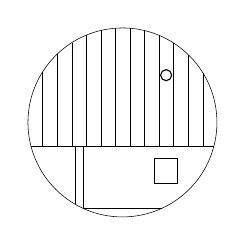
\begin{tikzpicture}
	
%camiseta
	\draw[black, very thin] (2,2) circle (12mm); 
	%%%%%%Camiseta lisa%%%%%	
	%\draw[black, thin] (2.555,2.6) circle (0.07cm); %Escudo
	%cuello

	%%%%%%%% 4 rayas verticales %%%%%%%
	%\draw[black, thin] (2.3,2.7) circle (0.07cm); %Escudo
	%%
	%\draw[black, line width=0.01mm](1.4,1.7)--(1.4,3.04);  %ultra thin, very thin
	%\draw[black, line width=0.01mm](2.0,1.7)--(2.0,3.2);  
	%\draw[black, line width=0.01mm](2.6,1.7)--(2.6,3.04);  

	%%%%%%% 5 rayas verticales %%%%%%%
	%\draw[black, thin] (2.464,2.7) circle (0.07cm); %Escudo
	%%
	%\draw[black, ultra thin](1.304,1.7)--(1.304,2.98);
	%\draw[black, ultra thin](1.768,1.7)--(1.768,3.18);  
	%\draw[black, ultra thin](2.232,1.7)--(2.232,3.18);  
	%\draw[black, ultra thin](2.696,1.7)--(2.696,2.98);  
	
	%%%%%%% 6 rayas verticales %%%%%%%
	%\draw[black, thin] (2.6,2.6) circle (0.07cm); %Escudo
	%%
	%\draw[black, ultra thin](1.2,1.7)--(1.2,2.89);  %ultra thin, very thin
	%\draw[black, ultra thin](1.6,1.7)--(1.6,3.13);  
	%\draw[black, ultra thin](2.0,1.7)--(2.0,3.2);  
	%\draw[black, ultra thin](2.4,1.7)--(2.4,3.13);  
	%\draw[black, ultra thin](2.8,1.7)--(2.8,2.89);  

	%%%%%%% 7 rayas verticales %%%%%%%
	%\draw[black, thin] (2.66286,2.6) circle (0.07cm); %Escudo
	%%
	%\draw[black, ultra thin](1.17143,1.7)--(1.17143,2.87);
	%\draw[black, ultra thin](1.50286,1.7)--(1.50286,3.09);  
	%\draw[black, ultra thin](1.83429,1.7)--(1.83429,3.19);  
	%\draw[black, ultra thin](2.16571,1.7)--(2.16571,3.19);  
	%\draw[black, ultra thin](2.49714,1.7)--(2.49714,3.09);
	%\draw[black, ultra thin](2.82857,1.7)--(2.82857,2.87);

	%%%%%%% 8 rayas verticales %%%%%%%
	%\draw[black, thin] (2.6,2.6) circle (0.07cm); %Escudo
	%%
	%\draw[black, ultra thin](1.13,1.7)--(1.13,2.89);  %ultra thin, very thin
	%\draw[black, ultra thin](1.42,1.7)--(1.42,3.13);  
	%\draw[black, ultra thin](1.71,1.7)--(1.71,3.2);  
	%\draw[black, ultra thin](2.0,1.7)--(2.0,3.13);  
	%\draw[black, ultra thin](2.29,1.7)--(2.29,2.89);
	%\draw[black, ultra thin](2.58,1.7)--(2.58,2.89);
	%\draw[black, ultra thin](2.87,1.7)--(2.87,2.89);
	
	
	%%%%%%% 12 rayas verticales %%%%%%%
	%\draw[black, thin] (2.5,2.6) circle (0.07cm); %Escudo
	%%
	%\draw[black, ultra thin](1,1.7)--(1,2.66);  %ultra thin, very thin
	%\draw[black, ultra thin](1.2,1.7)--(1.2,2.89); 
	%\draw[black, ultra thin](1.4,1.7)--(1.4,3.04); 
	%\draw[black, ultra thin](1.6,1.7)--(1.6,3.13); 
	%\draw[black, ultra thin](1.8,1.7)--(1.8,3.18); 
	%\draw[black, ultra thin](2.0,1.7)--(2.0,3.2); 
	%\draw[black, ultra thin](2.2,1.7)--(2.2,3.18); 
	%\draw[black, ultra thin](2.4,1.7)--(2.4,3.13); 
	%\draw[black, ultra thin](2.6,1.7)--(2.6,3.04); 
	%\draw[black, ultra thin](2.8,1.7)--(2.8,2.89); 
	%\draw[black, ultra thin](3.0,1.7)--(3.0,2.66); 
	
	%%%%%%% 13 rayas verticales %%%%%%%
	\draw[black, thin] (2.555,2.6) circle (0.07cm); %Escudo
	%
	\draw[black, ultra thin](0.985,1.7)--(0.985,2.64); %ultra thin, very thin
	\draw[black, ultra thin](1.170,1.7)--(1.170,2.865); 
	\draw[black, ultra thin](1.355,1.7)--(1.355,3.013); 
	\draw[black, ultra thin](1.540,1.7)--(1.540,3.108); 
	\draw[black, ultra thin](1.725,1.7)--(1.725,3.171); 
	\draw[black, ultra thin](1.910,1.7)--(1.910,3.2); 
	\draw[black, ultra thin](2.095,1.7)--(2.095,3.2); 
	\draw[black, ultra thin](2.280,1.7)--(2.280,3.168); 
	\draw[black, ultra thin](2.465,1.7)--(2.465,3.105); 
	\draw[black, ultra thin](2.650,1.7)--(2.650,3.01); 
	\draw[black, ultra thin](2.835,1.7)--(2.835,2.861); 
	\draw[black, ultra thin](3.020,1.7)--(3.020,2.633); 

	
%pantal�n
	\draw[black, ultra thin] (0.84,1.7) -- (3.16,1.7);
	%Raya vertical doble
	\draw[black, ultra thin] (1.4,0.96) -- (1.4,1.7); \draw[black, ultra thin] (1.5,0.91) -- (1.5,1.7); 
	%N�mero
	%\node at (2.555,1.4) {$\mathbbm{2}$};
	\draw[black, ultra thin] (2.4,1.23) rectangle (2.7,1.55);
	
%medias
	\draw[black, ultra thin] (1.5,0.91) -- (2.503,0.91);
	%\draw[black, very thin] (1.568,0.88) -- (2.432,0.88);
\end{tikzpicture}
}

\newcommand{\filatrajes}[1][]{
\noindent\traje{}
\traje{}
\traje{}
\traje{}
\traje{}
\traje{}
\traje{}

\medskip
}

%Dibuja los trajes en la hoja
\filatrajes{}
\filatrajes{}
\filatrajes{}
\filatrajes{}
\filatrajes{}
\filatrajes{}
\filatrajes{}
\filatrajes{}
\filatrajes{}
\filatrajes{}

\end{document}
